\documentclass[10pt,firamath,cours]{nsi}
\begin{document}
\setcounter{chapter}{12}
\chapter{Arbres binaires de recherche}
\section{Principe}
\begin{definition}[]
    Un arbre binaire de recherche est un arbre binaire
    \begin{itemize}
        \item dont tous les n\oe uds comportent des valeurs du même type qu'il est possible de comparer (entiers, flottants, chaînes de caractères...) ;
        \item dont les valeurs de tous les n\oe uds situés dans le \textit{sous-arbre gauche} d'un n\oe ud sont \textit{inférieures ou égales} à la valeur de ce n\oe ud ;
    \end{itemize}   
\end{definition}
\begin{exemple}[s]
    Voici un ABR :
    \begin{center}
    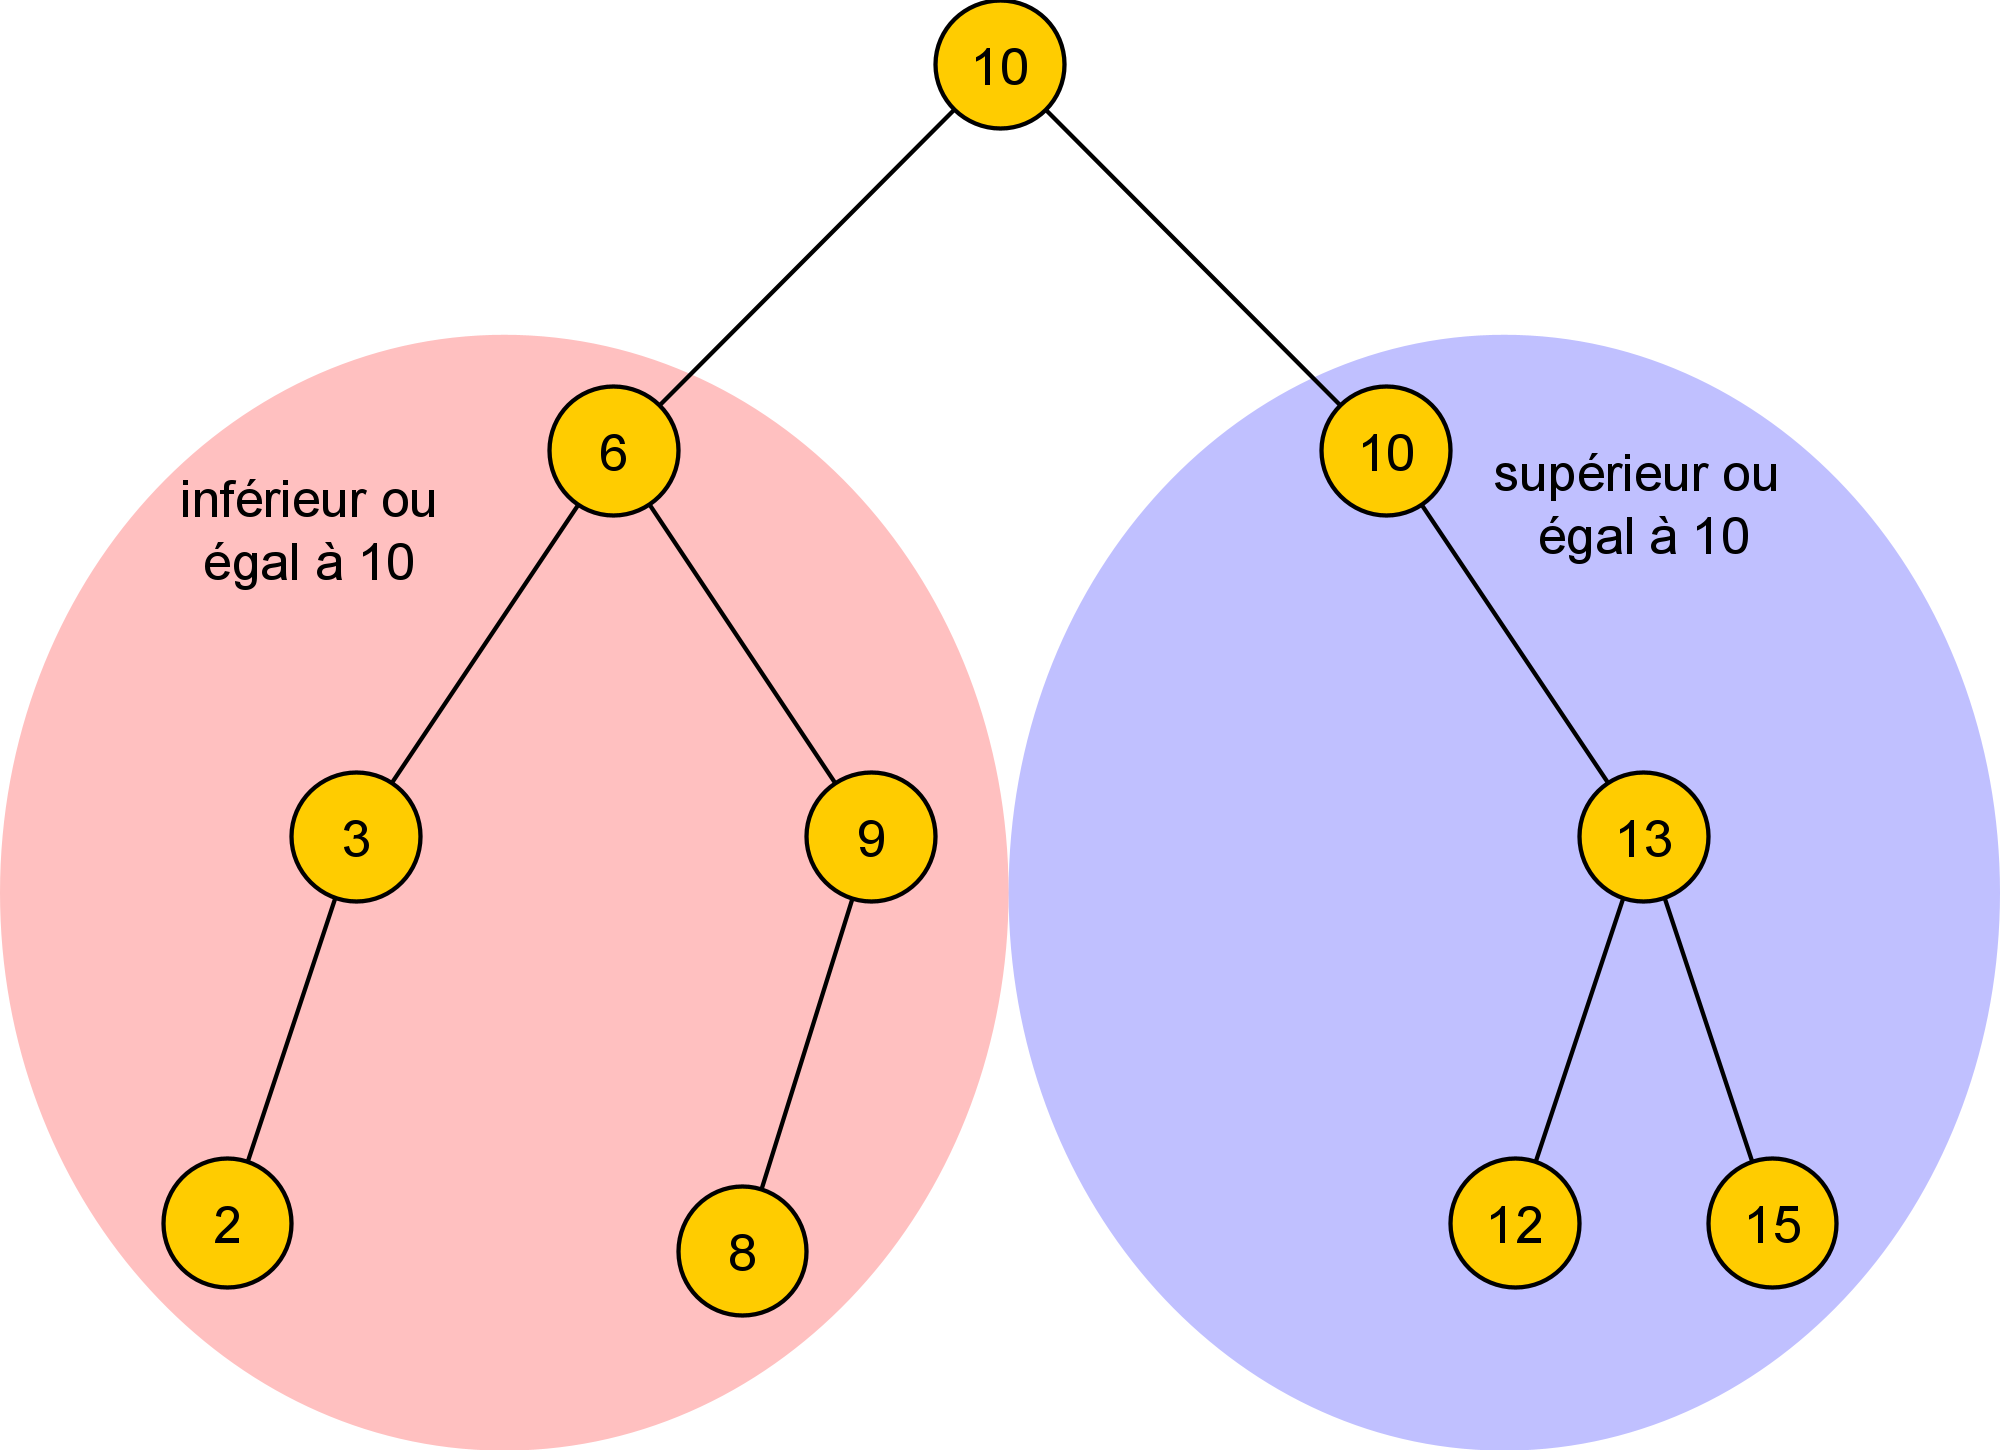
\includegraphics[width=7cm]{img/abr1}
    \end{center} 
    Ceci n'est pas un ABR
    \begin{center}
        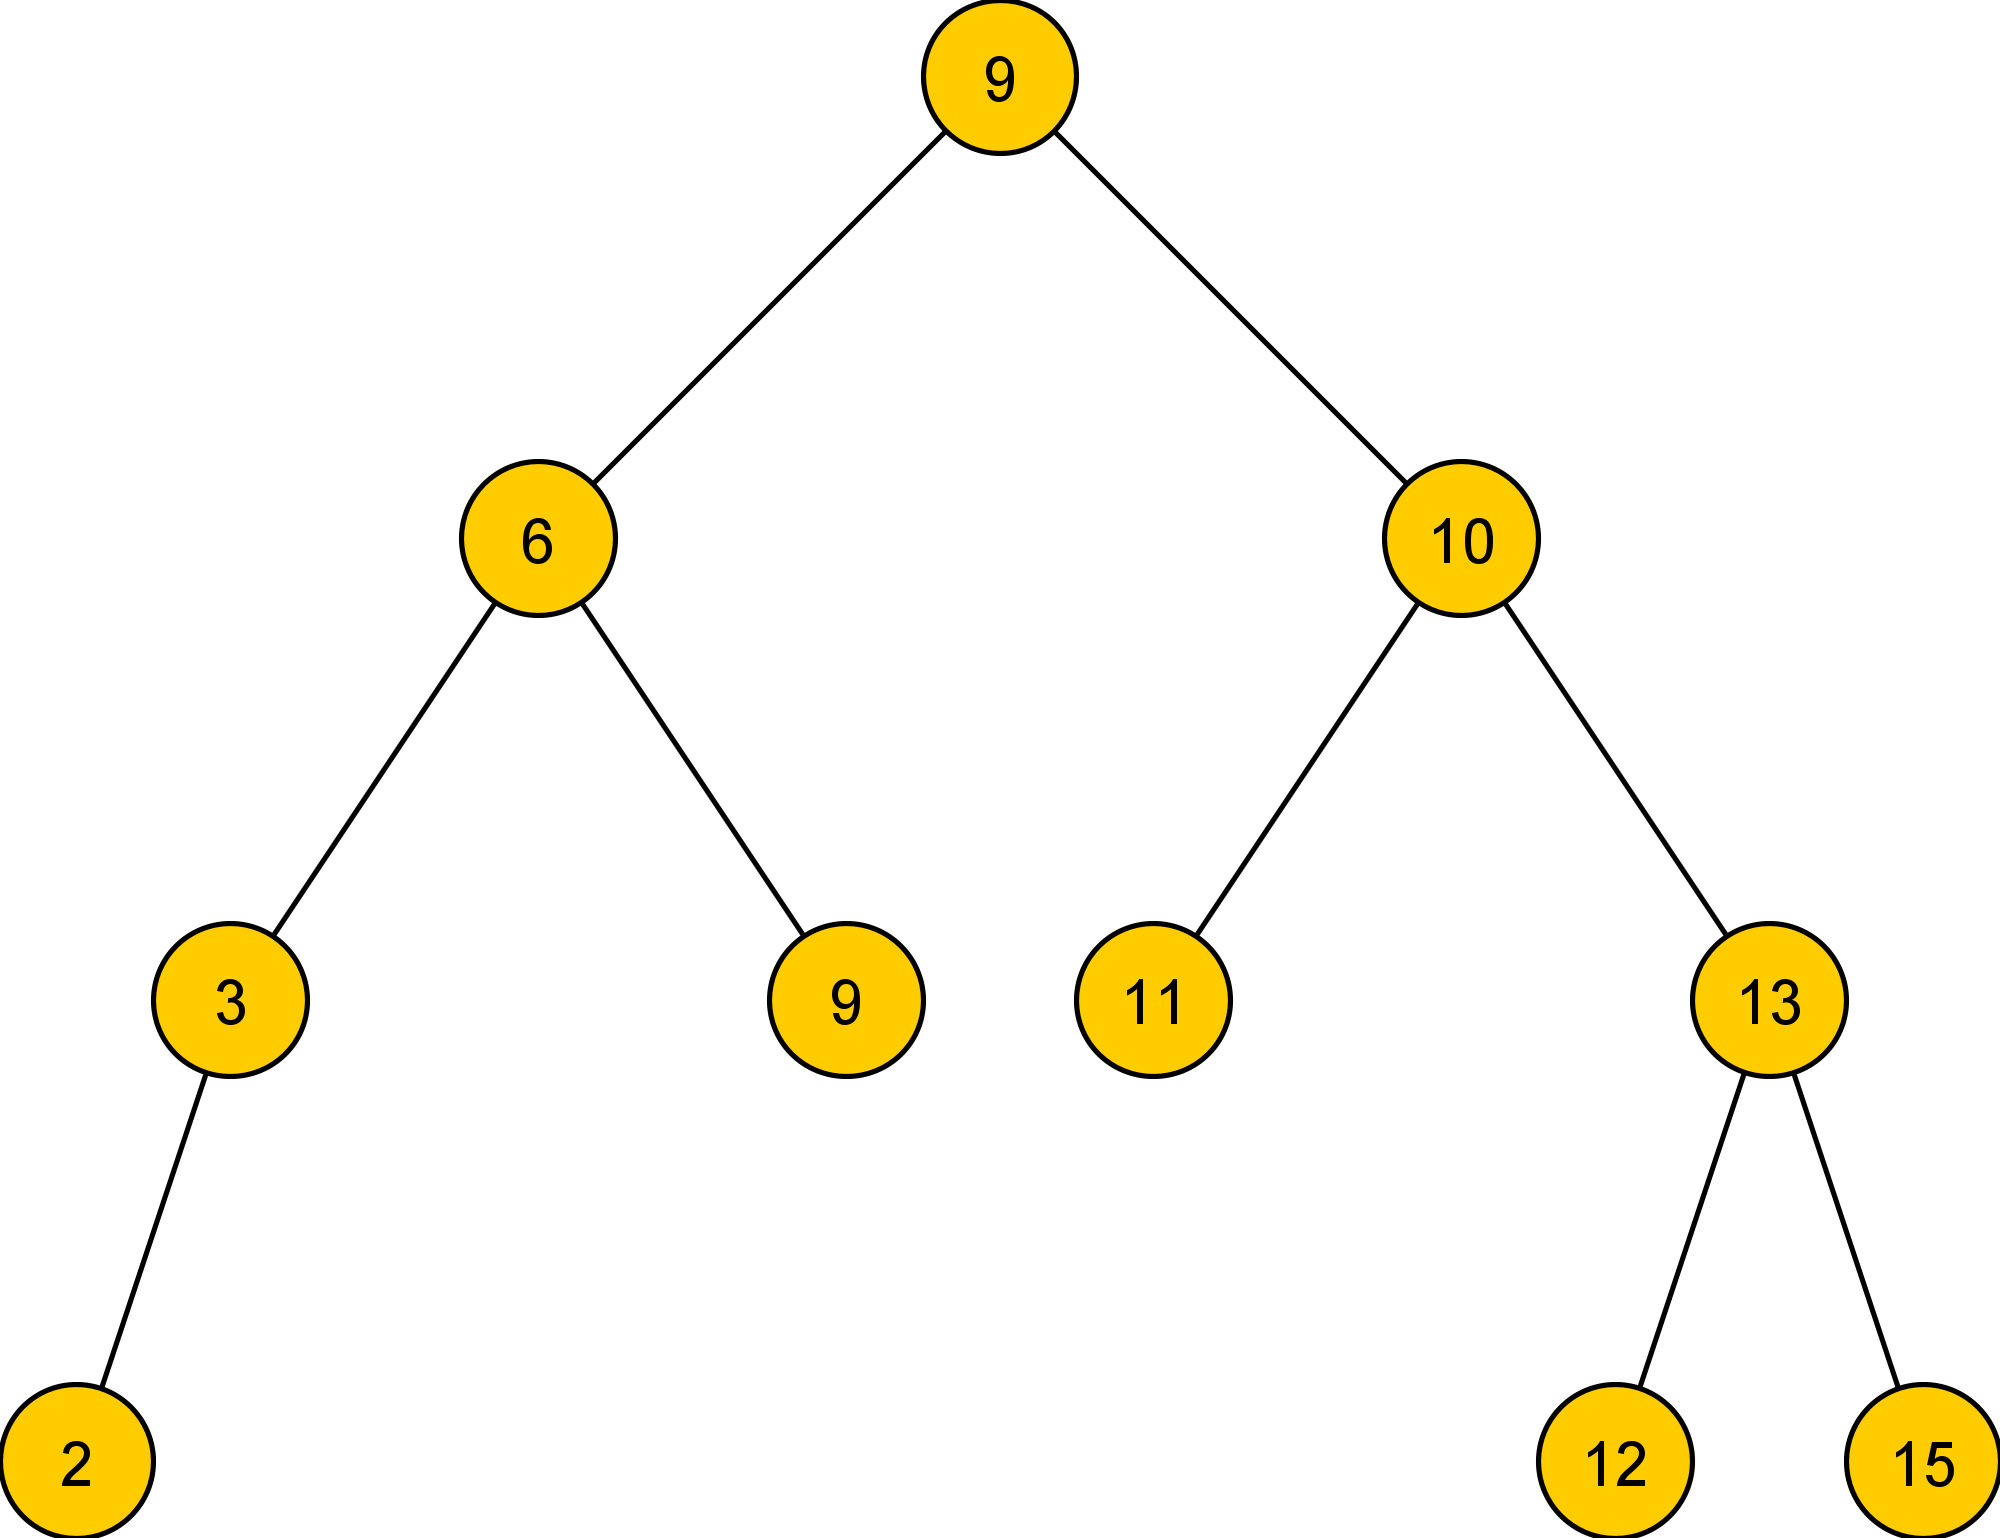
\includegraphics[width=5cm]{img/abr2}
    \end{center}
    En effet le nœud de valeur 11 n'est pas à la bonne place.
\end{exemple}

\begin{methode}[ : Recherche dans un ABR]
    On compare l'élément à trouver avec la valeur de la racine, puis selon les cas
    \begin{itemize}
        \item on s'arrête si on a trouvé la valeur ;
        \item on essaie d'aller à gauche si la l'élément est plus petit ;
        \item on essaie à droite s'il est plus grand ;
        \item si on ne peut continuer, on s'arrête et l'élément ne figure pas dans l'arbre.
    \end{itemize}
        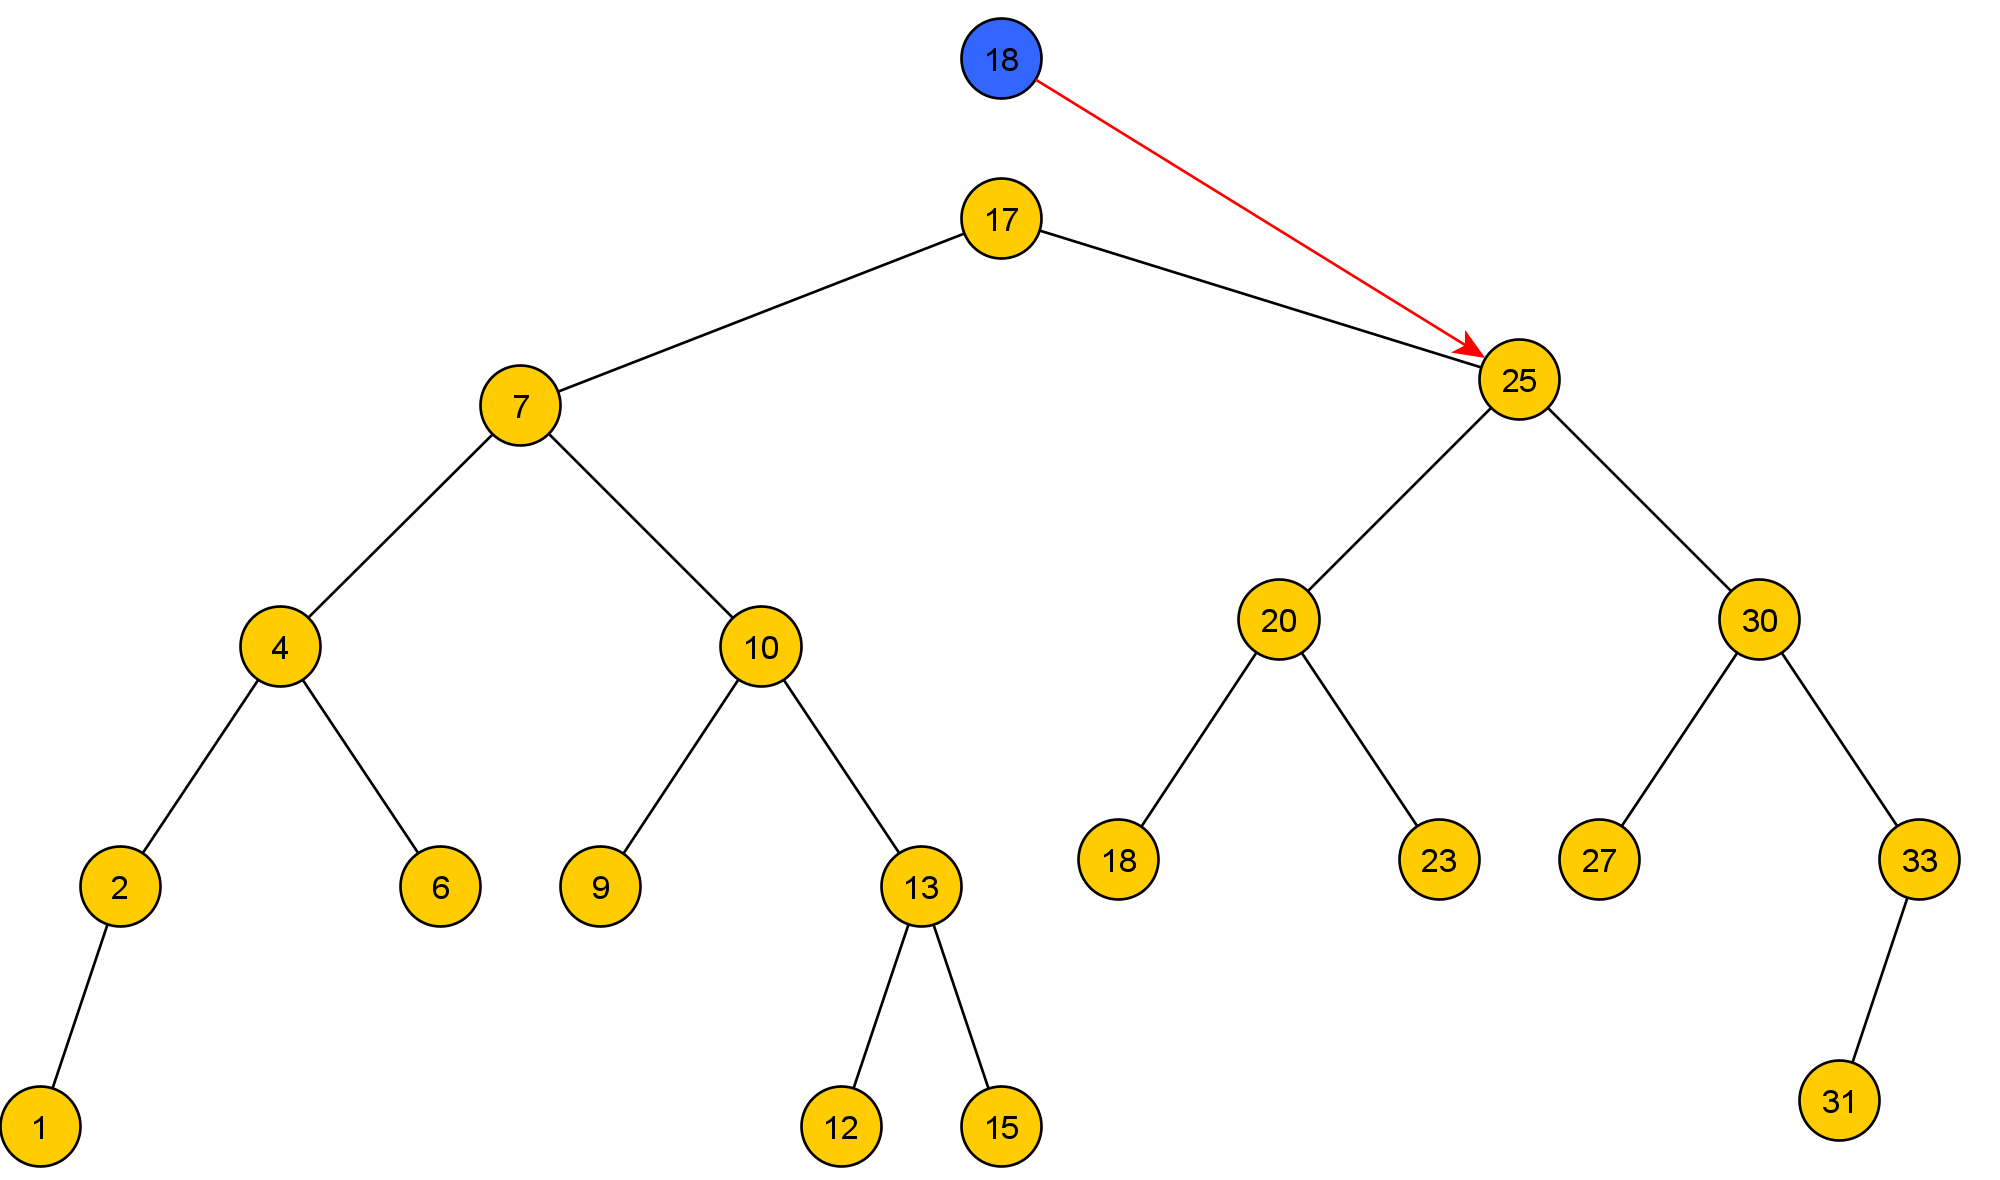
\includegraphics[width=6cm]{img/Recherche/recherche1} \hspace{2em}
        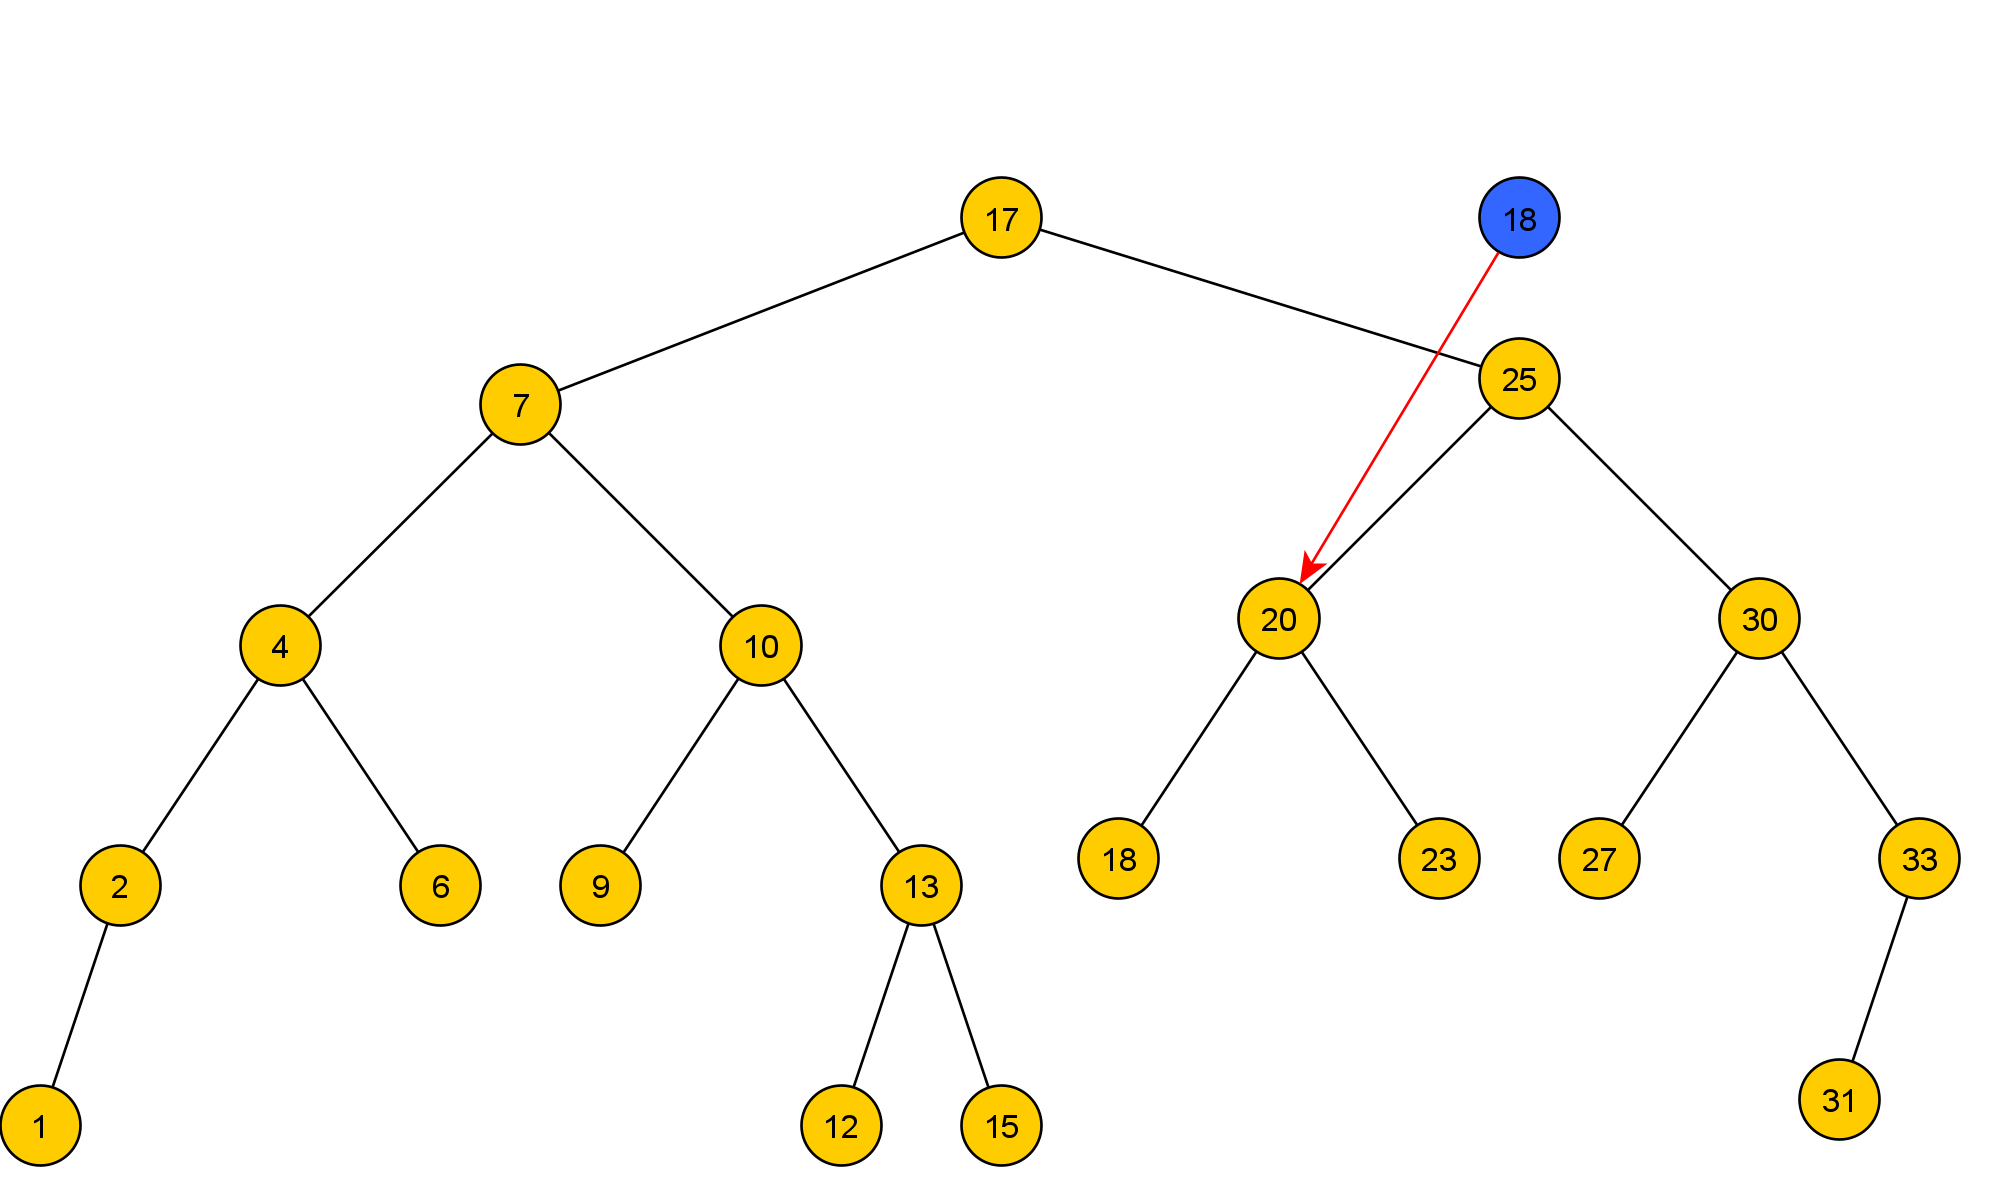
\includegraphics[width=6cm]{img/Recherche/recherche2}\\ 
        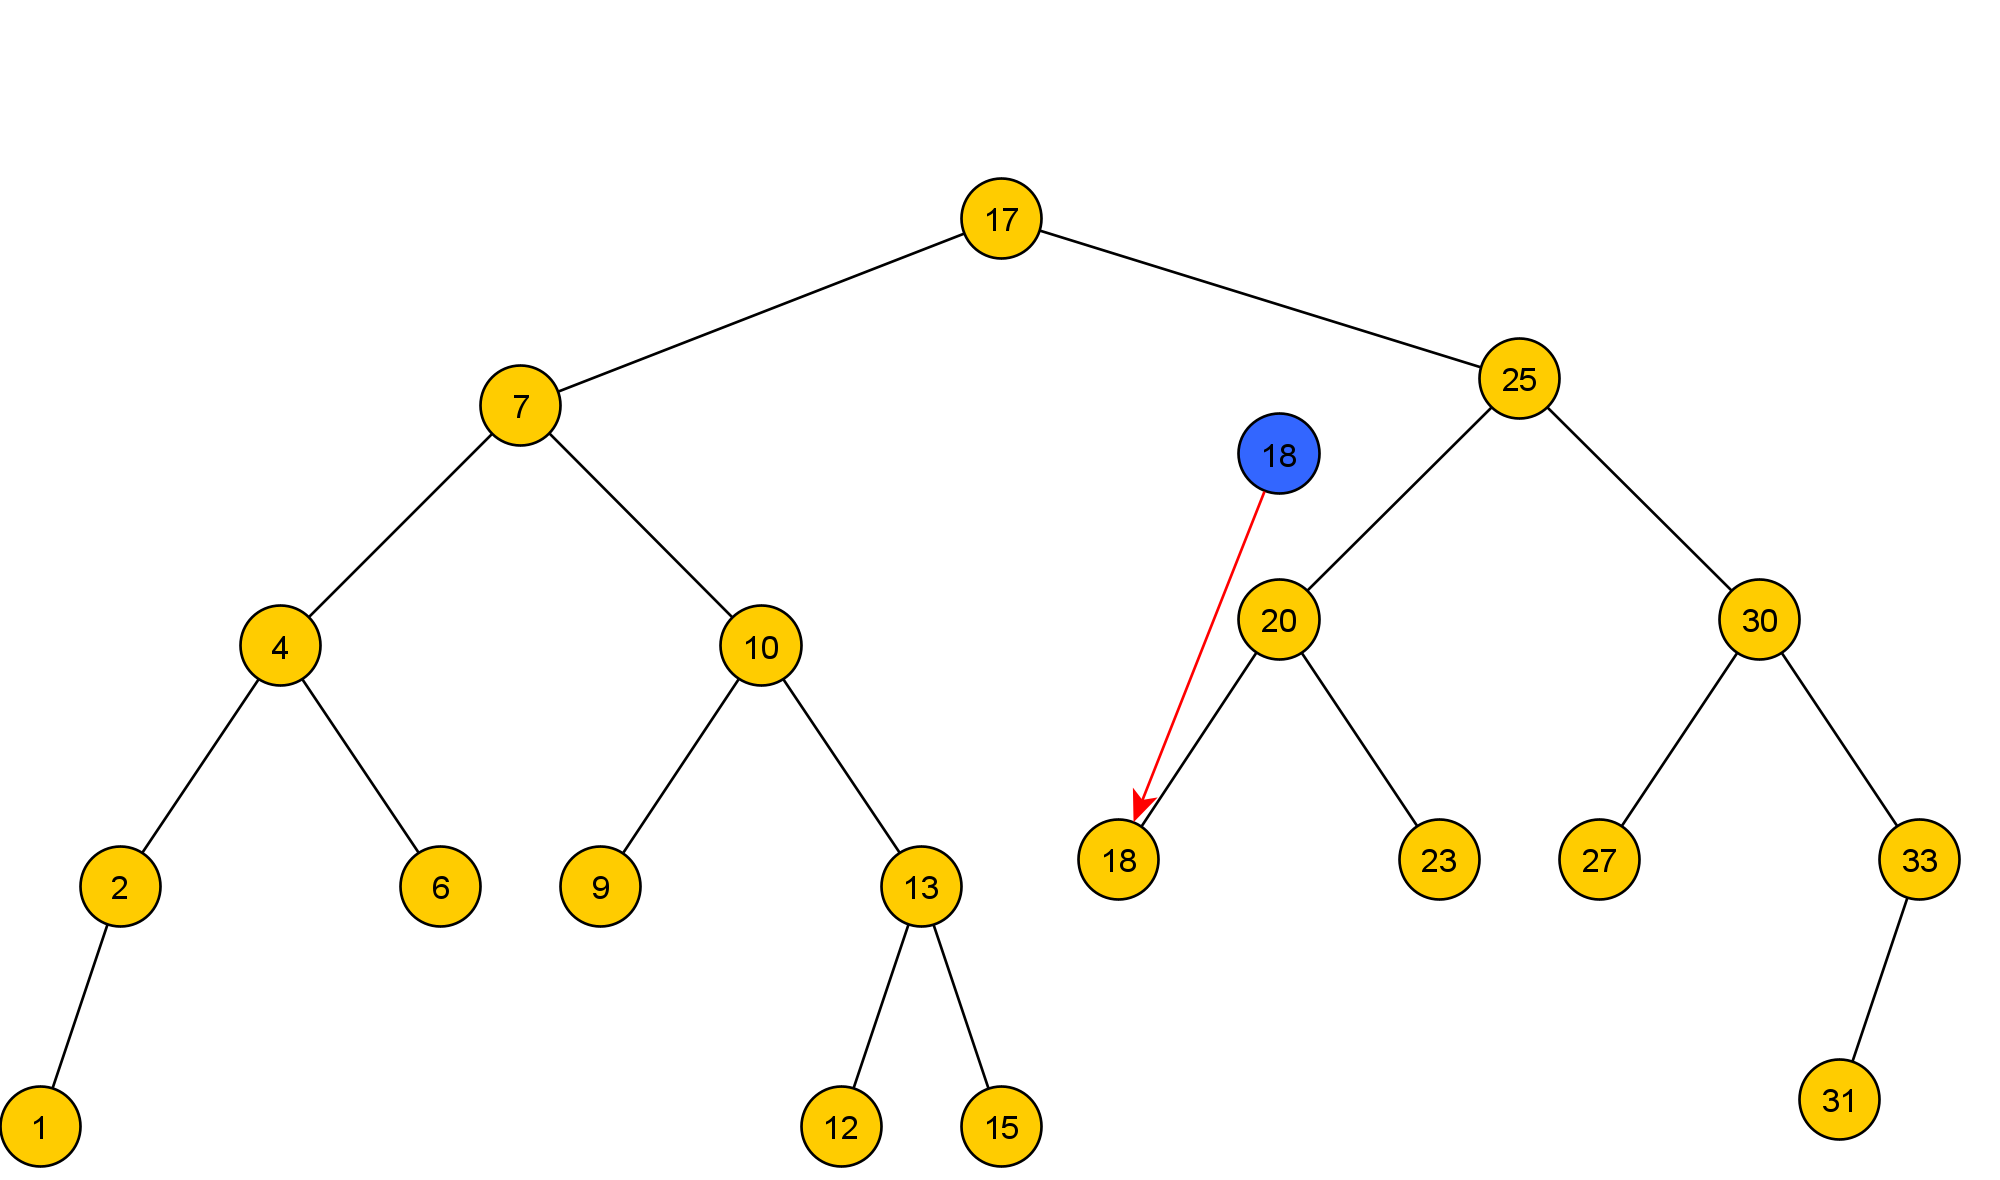
\includegraphics[width=6cm]{img/Recherche/recherche3} \hspace{2em}
        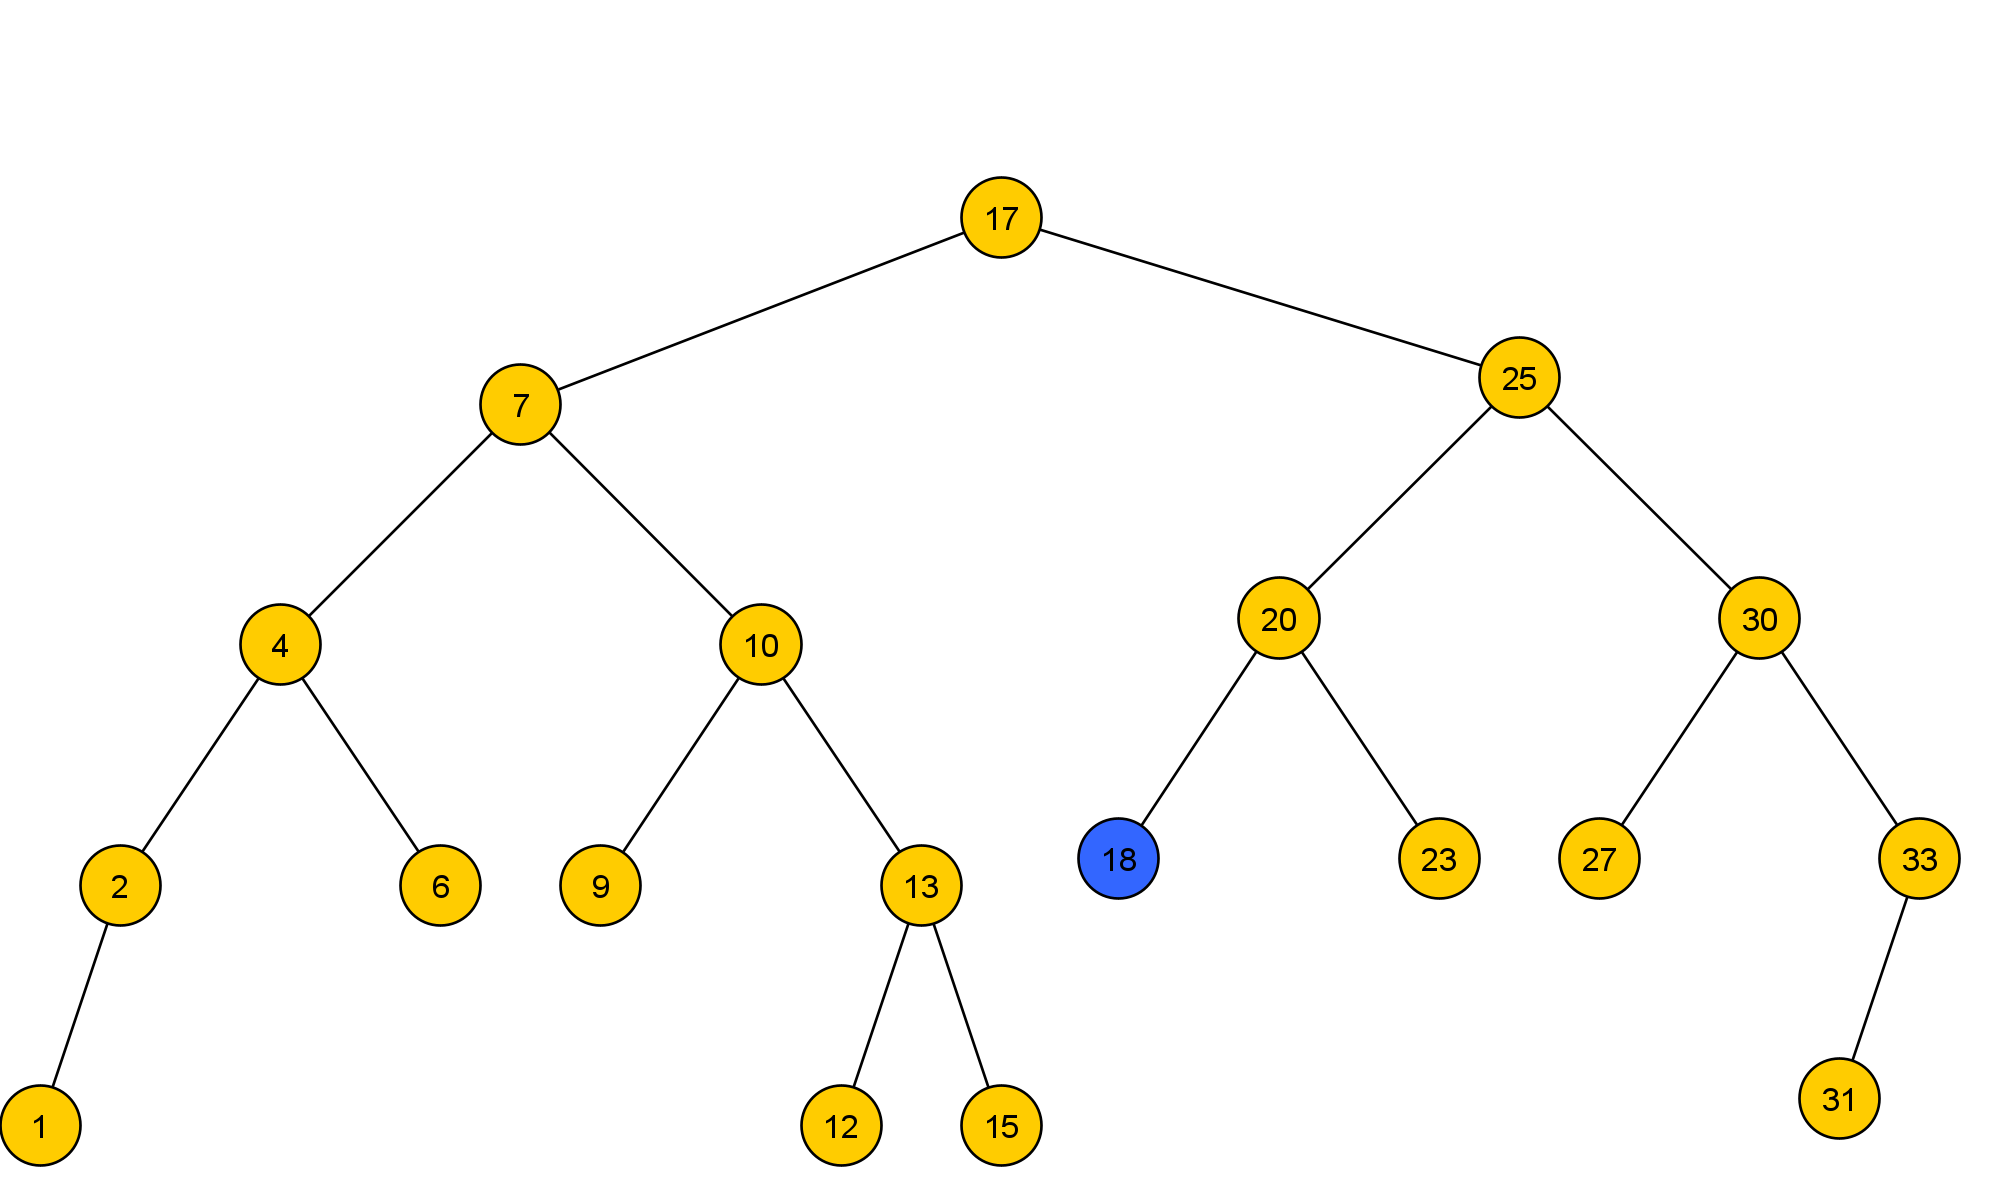
\includegraphics[width=6cm]{img/Recherche/recherche4}
\end{methode}

\begin{methode}[Ajout d'un élément dans un ABR]
    Le principe est le même que précédemment, quand on ne peut plus continuer, on crée une nouvelle feuille.\\
    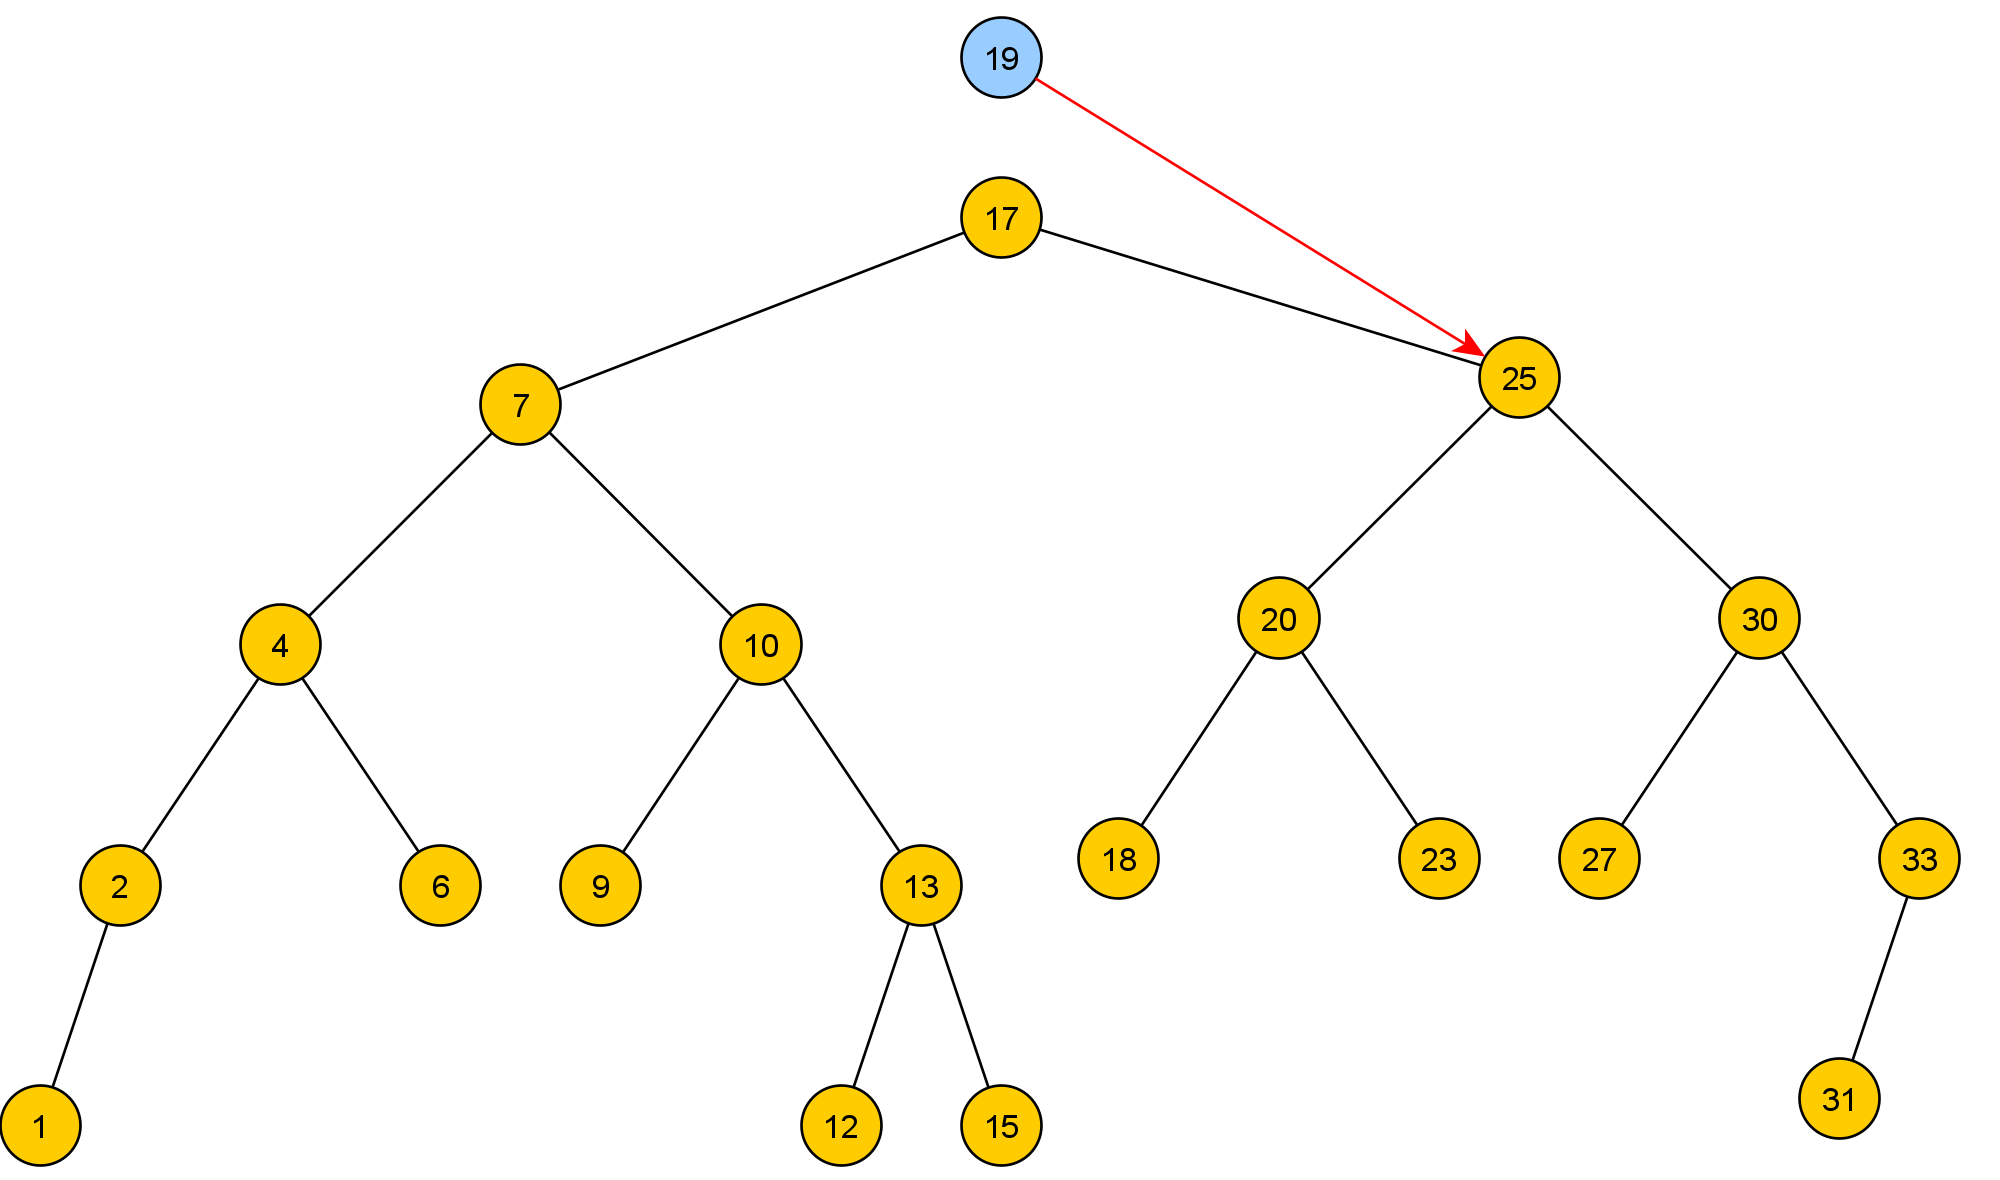
\includegraphics[width=6cm]{img/ajout/ajout1} \hspace{2em}
    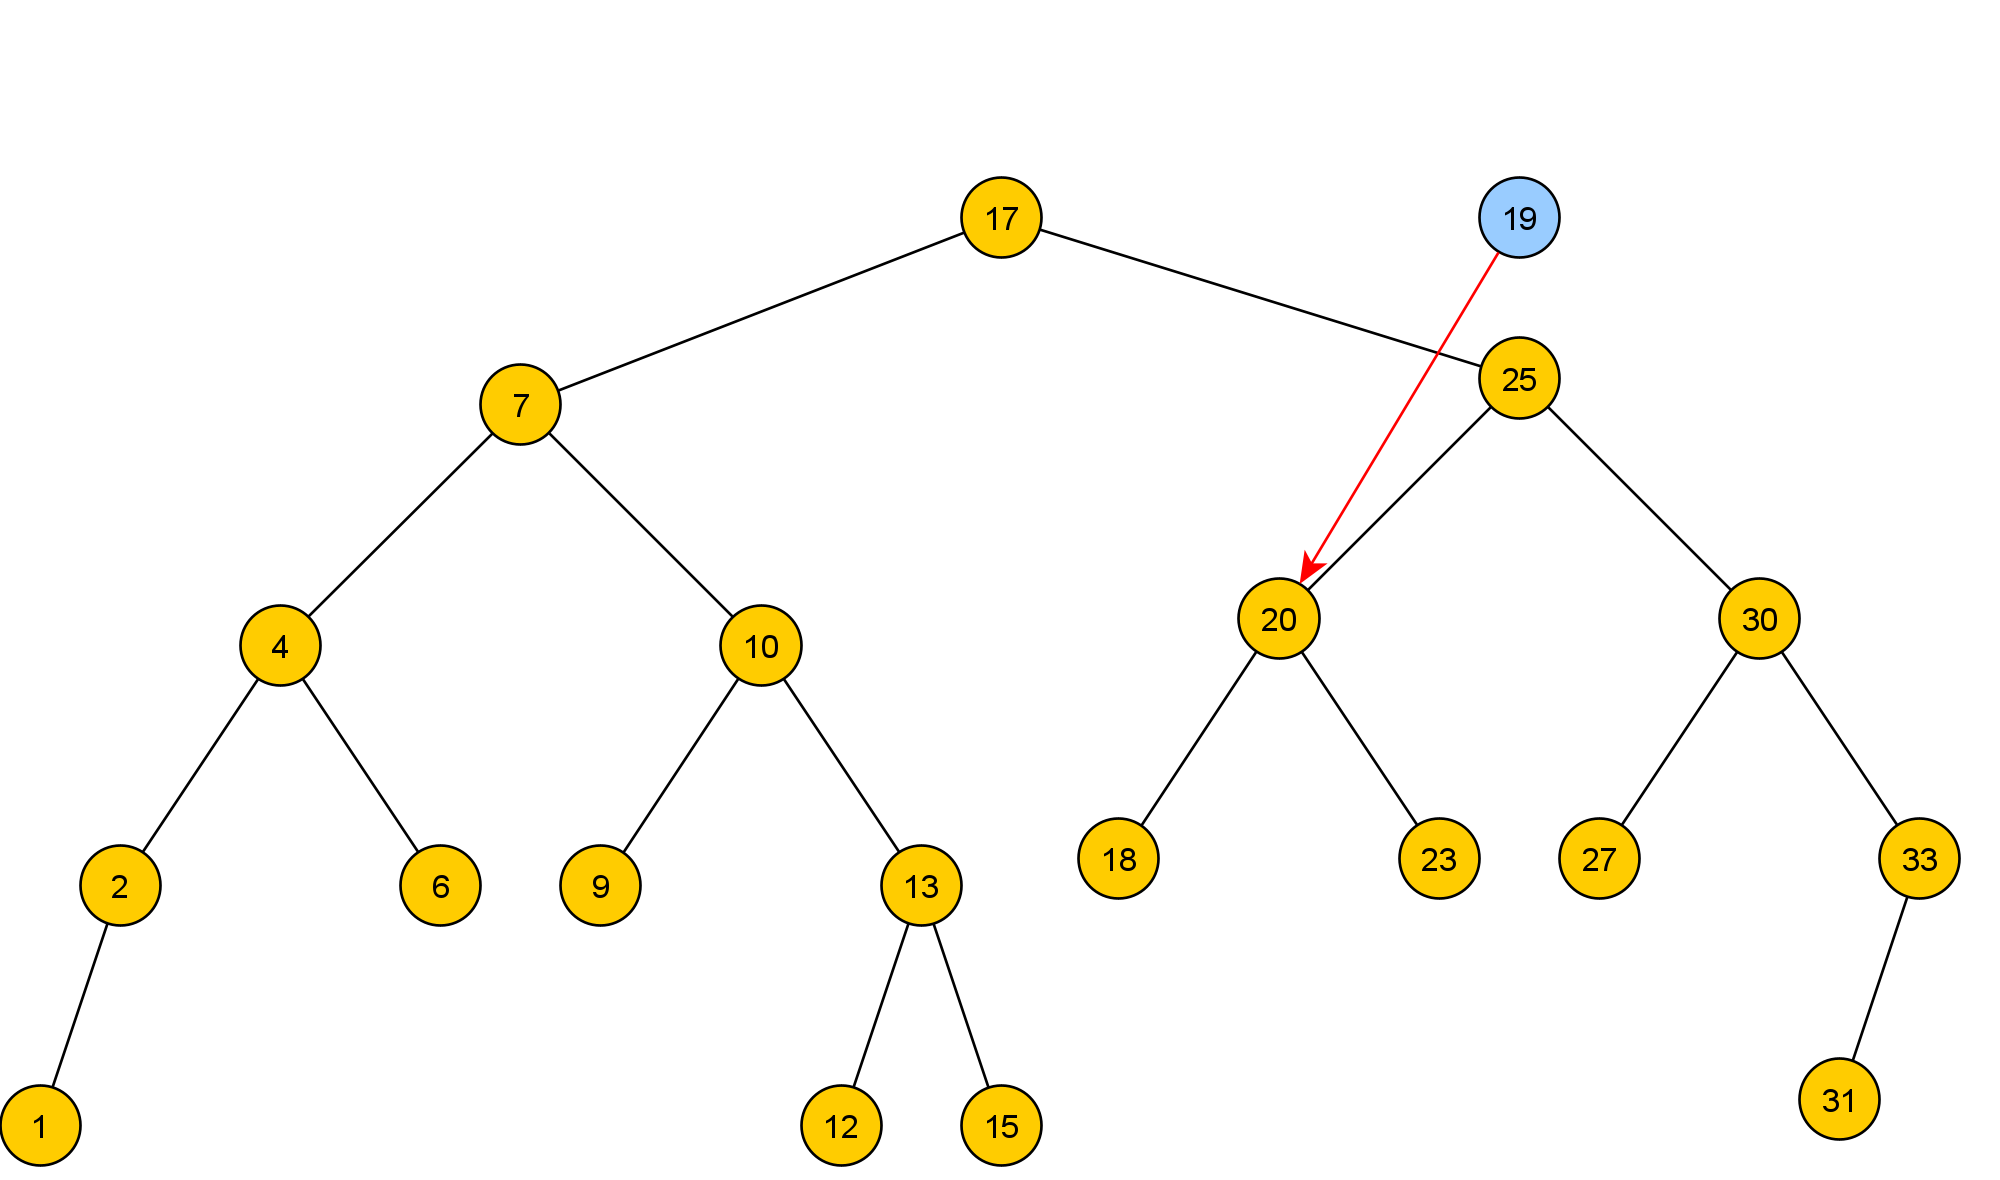
\includegraphics[width=6cm]{img/ajout/ajout2}\\ 
    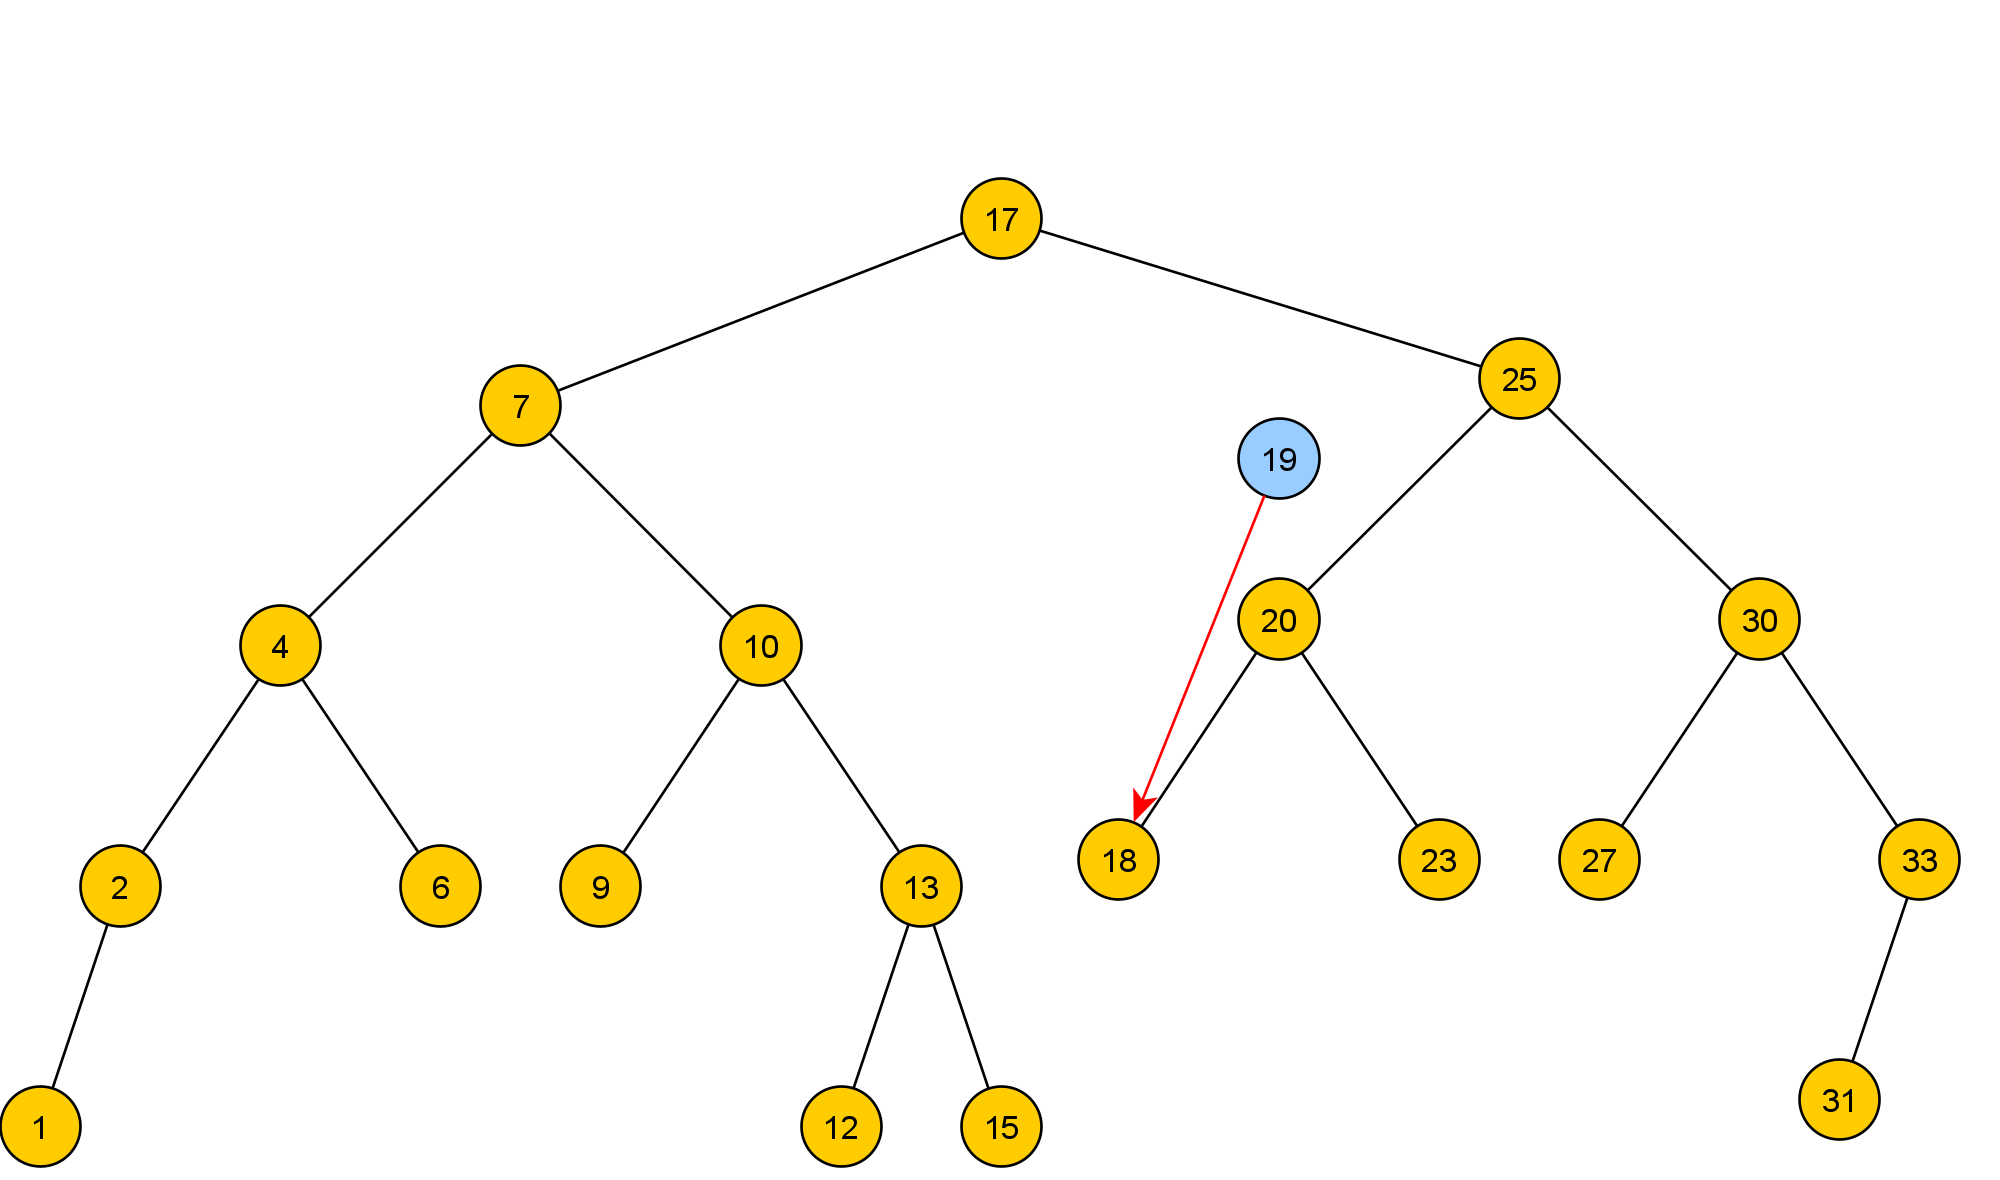
\includegraphics[width=6cm]{img/ajout/ajout3} \hspace{2em}
    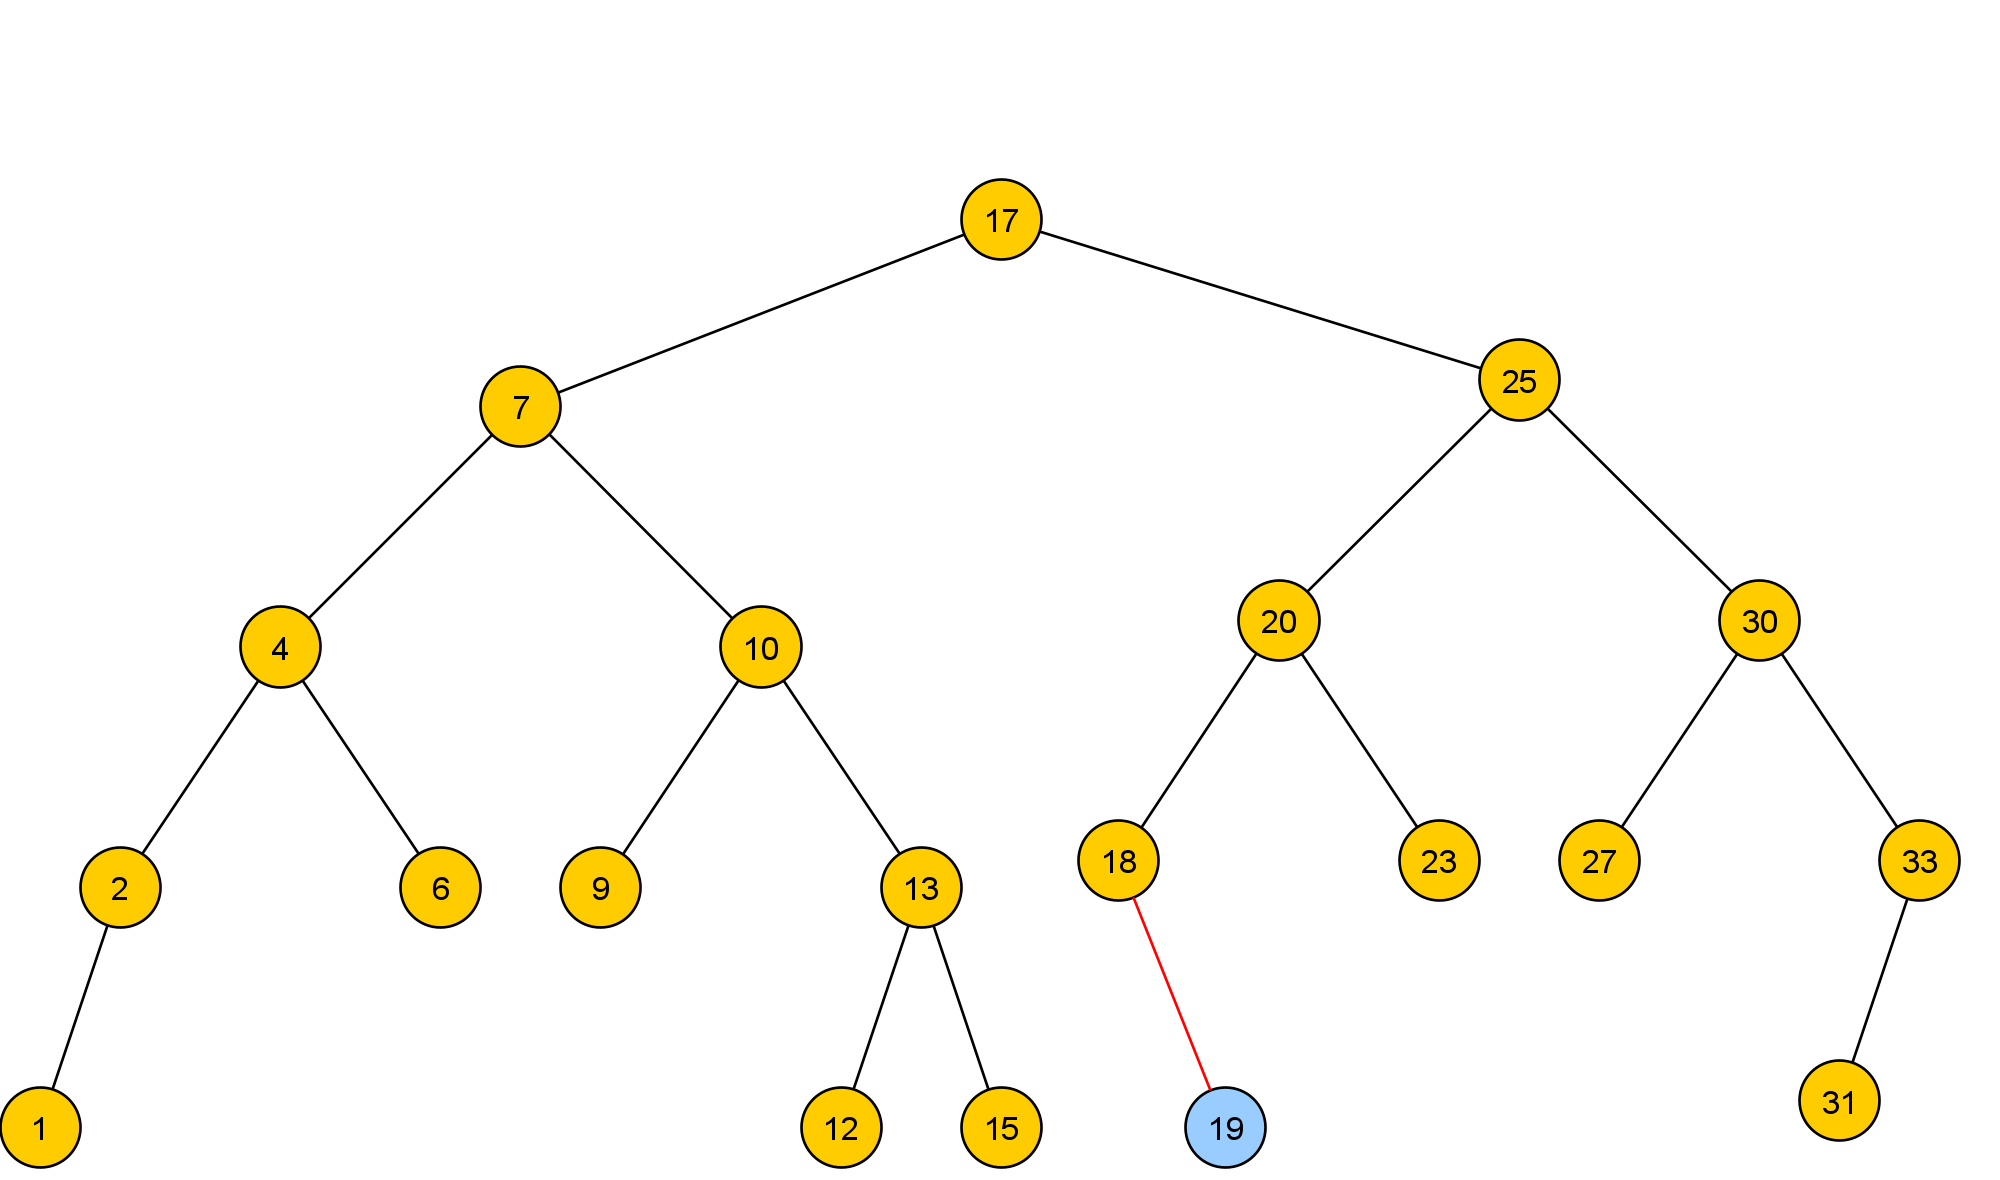
\includegraphics[width=6cm]{img/ajout/ajout4}  
\end{methode}

\begin{methode}[Suppression d'un élément dans un ABR (hors programme)]
    D'abord on cherchye le n\oe ud contenant l'élément.Si ce n'est pas une feuille, on le remplace par le maximum de son sous-arbre gauche ou par le minimum de son sous-arbre droit en enlevant ce dernier.\\
    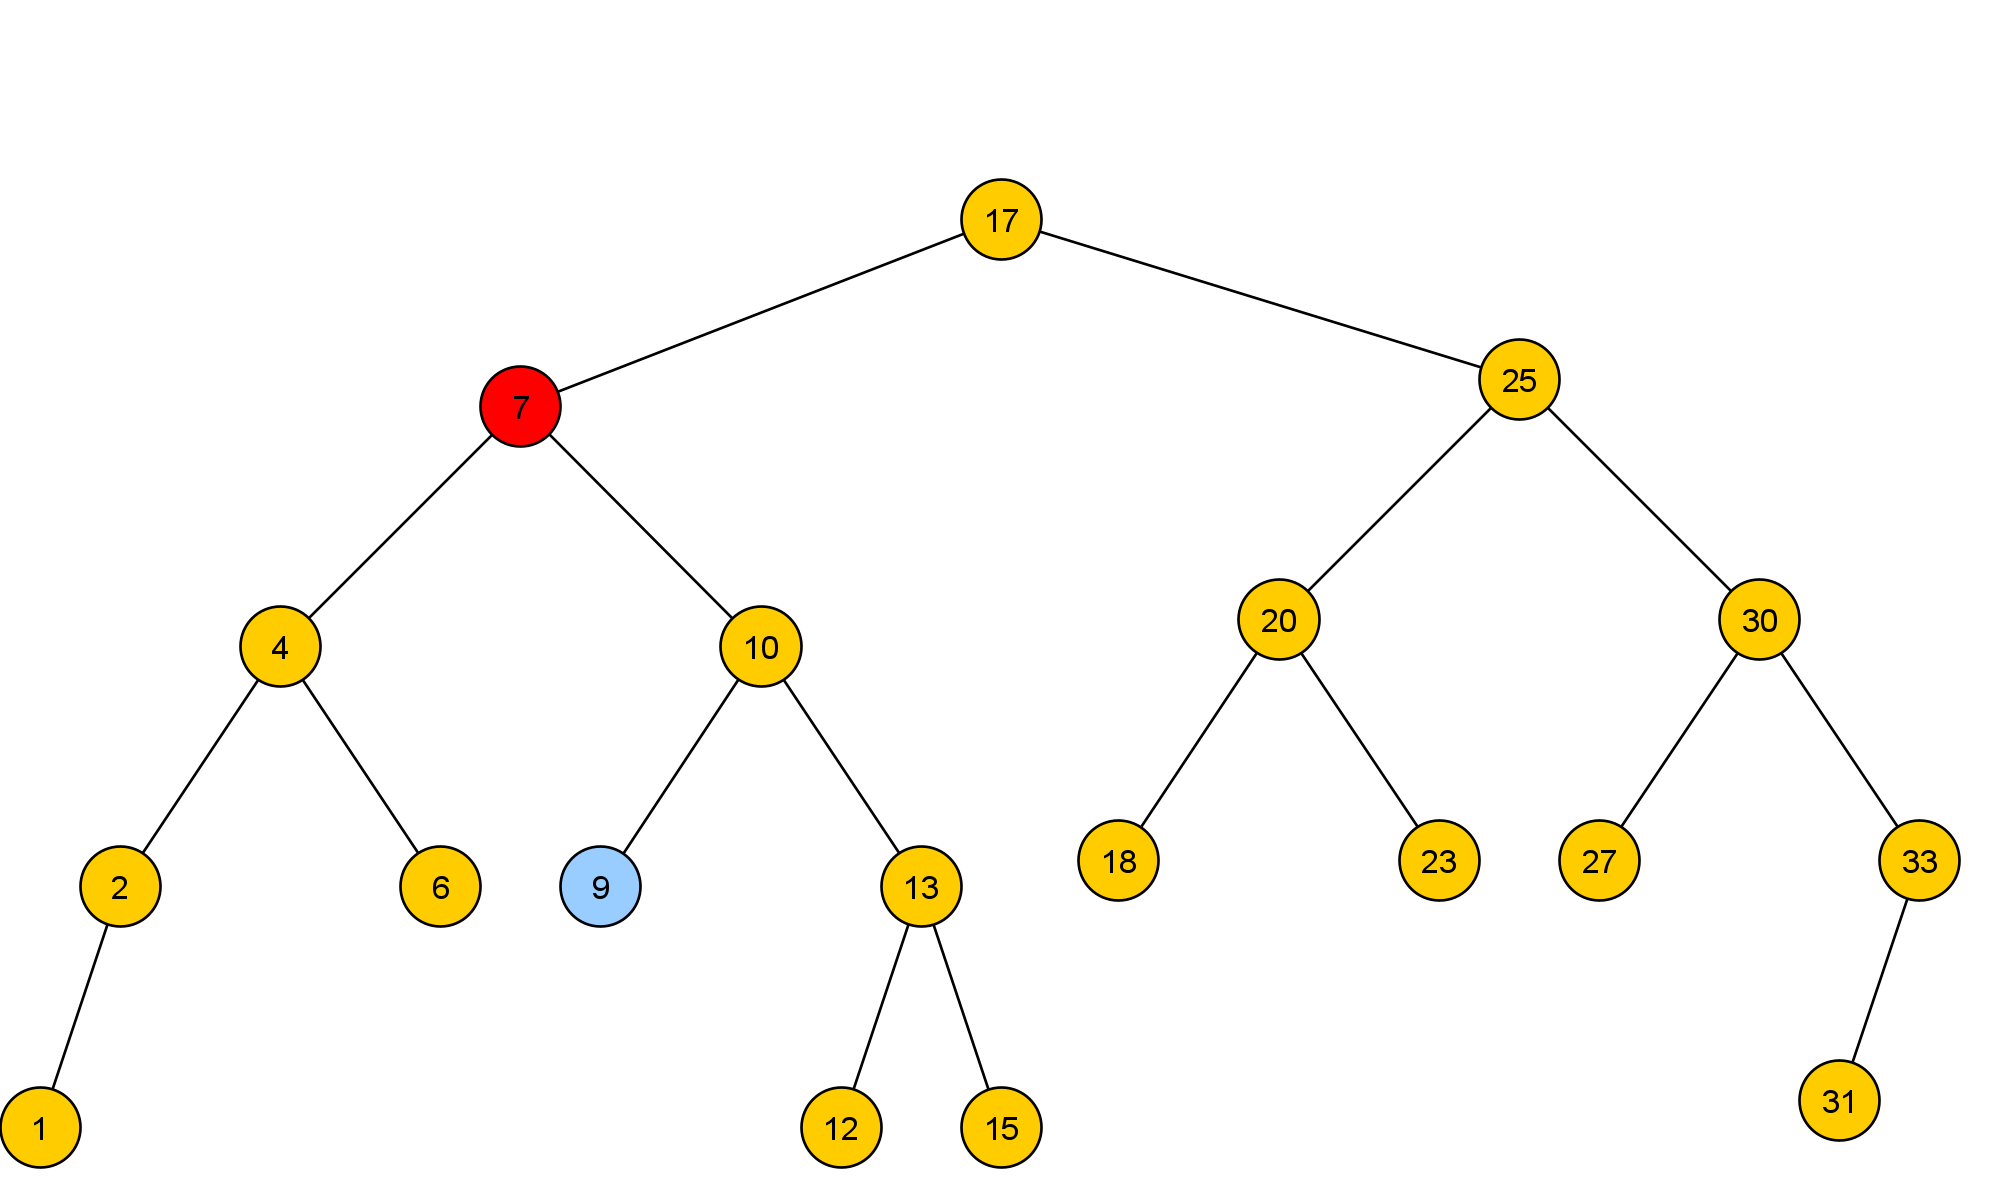
\includegraphics[width=6cm]{img/suppr/suppr1} \hspace{2em}
    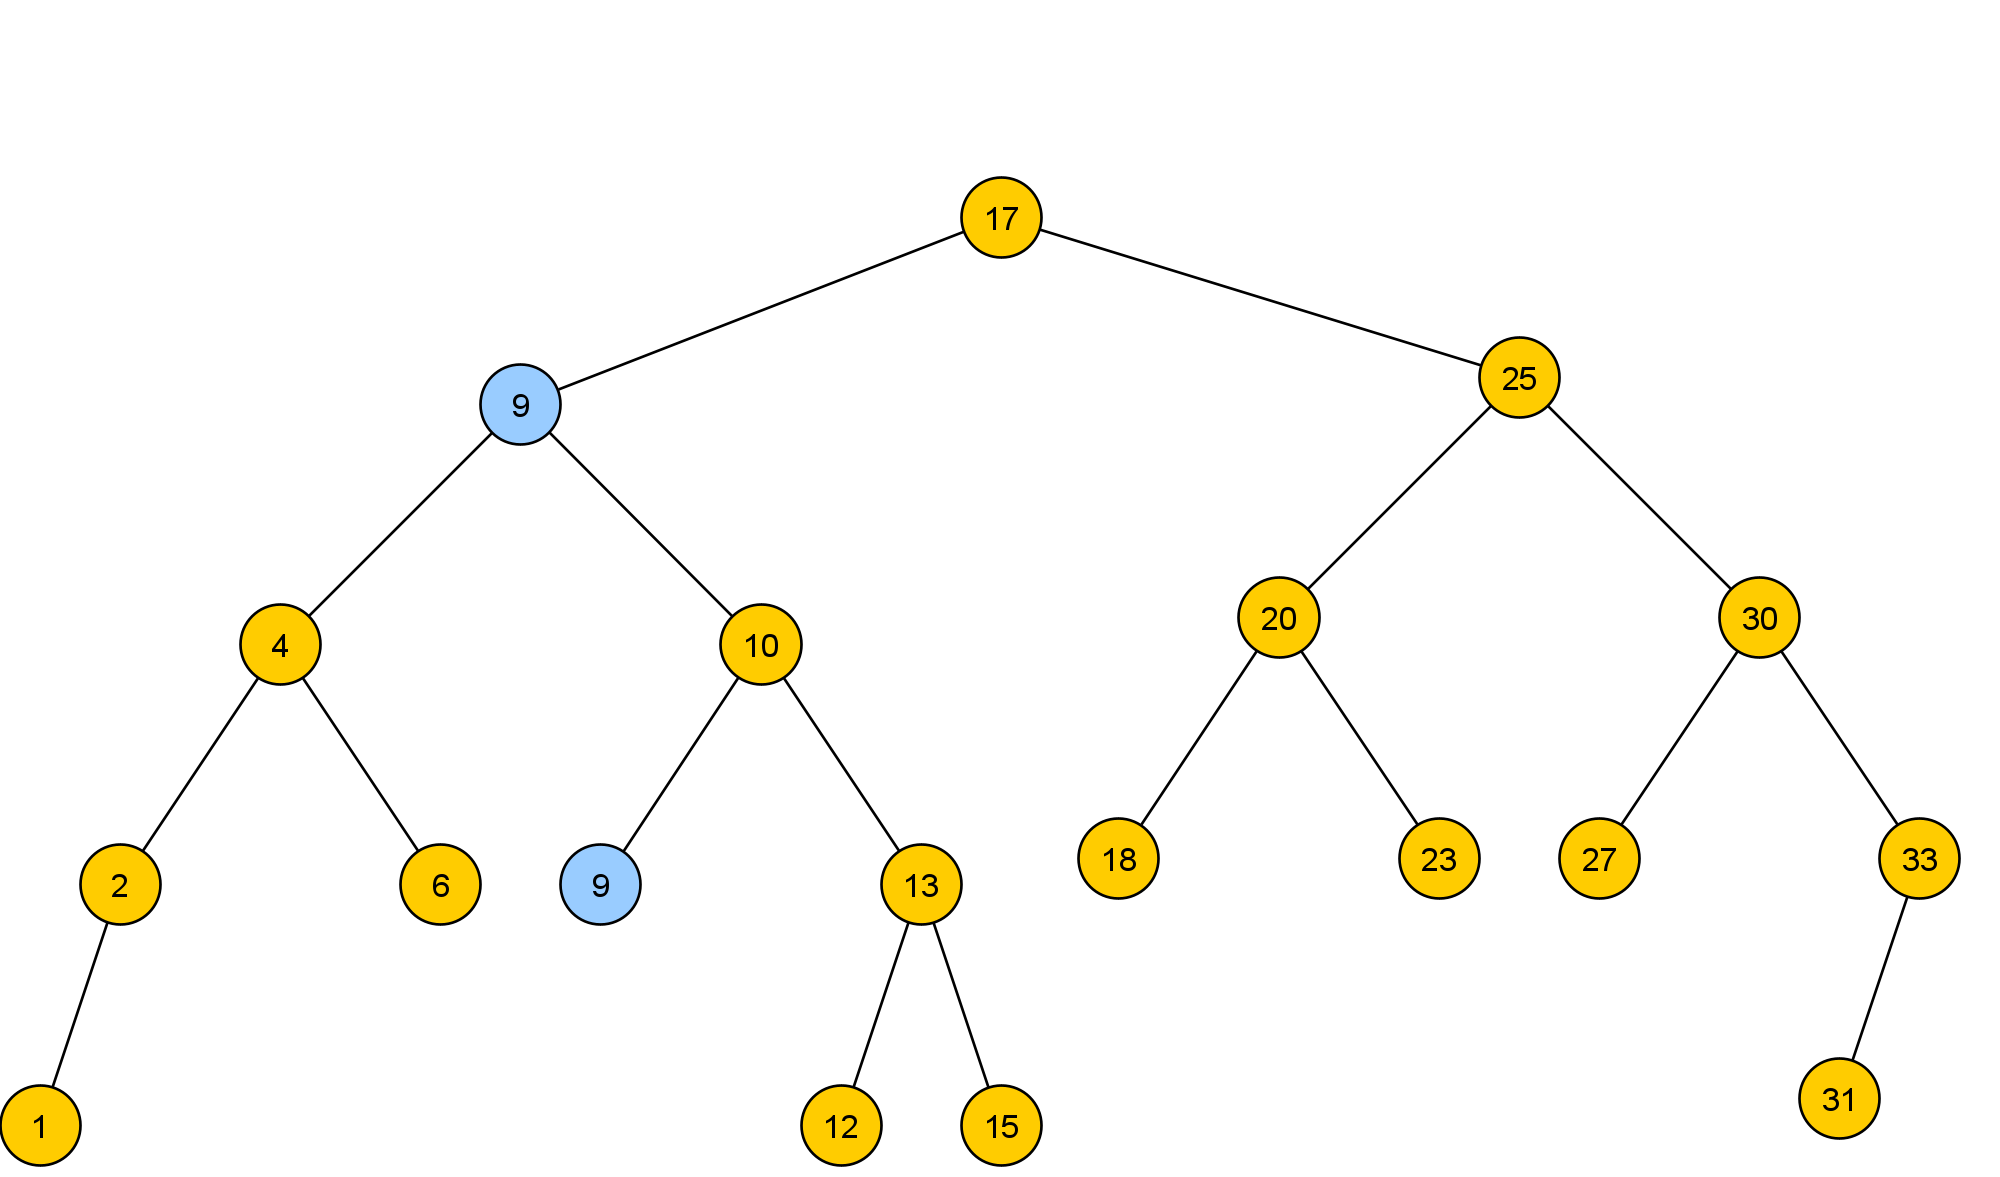
\includegraphics[width=6cm]{img/suppr/suppr2}
\end{methode}
\section{Intérets}

Le coût de recherche ou d'ajout d'un élément dans un ABR est proportionnel à sa hauteur.\\

Dans le pire des cas, où l'ABR est dégénéré, on ne gagne pas grand chose par rapport à une liste.\\

Le meilleur des cas serait d'avoir un arbre parfait.\\

Il existe des méthodes pour, lors de l'ajout  d'un élément dans un ABR, s'assurer que celui-ci reste bien \textit{équilibré}. Elles ne sont pas au programme de terminale.

Dans ce cas la hauteur $h$ de l'ABR est dite \textit{logarithmique}, c'est à dire que si $N$ désigne le nombre de n\oe uds, il existe une constante $C$ telle que 
$$h\leqslant C.\log_2(N)$$
Alors, avec un ABR équilibré, les opérations de recherche et d'ajouts sont très efficaces.

\begin{exemple}[]
    Imaginons un ABR parfait de hauteur $h$, il possède $N=2^{h+1}-1$ éléments.\\
    Le temps de recherche ou d'ajout d'un élément (dans le pire des cas) est de l'ordre de $h$.\\
    
    Prenons $h=50$, alors notre ABR comporte \np{2251799813685247} éléments, et on trouve ou on ajoute un nouvel élément en 51 étapes au maximum ! 
\end{exemple}


\end{document}